\documentclass{article}
\usepackage[utf8]{inputenc}
\usepackage{fullpage}
\usepackage{tikz}


\begin{document}
\begin{center}

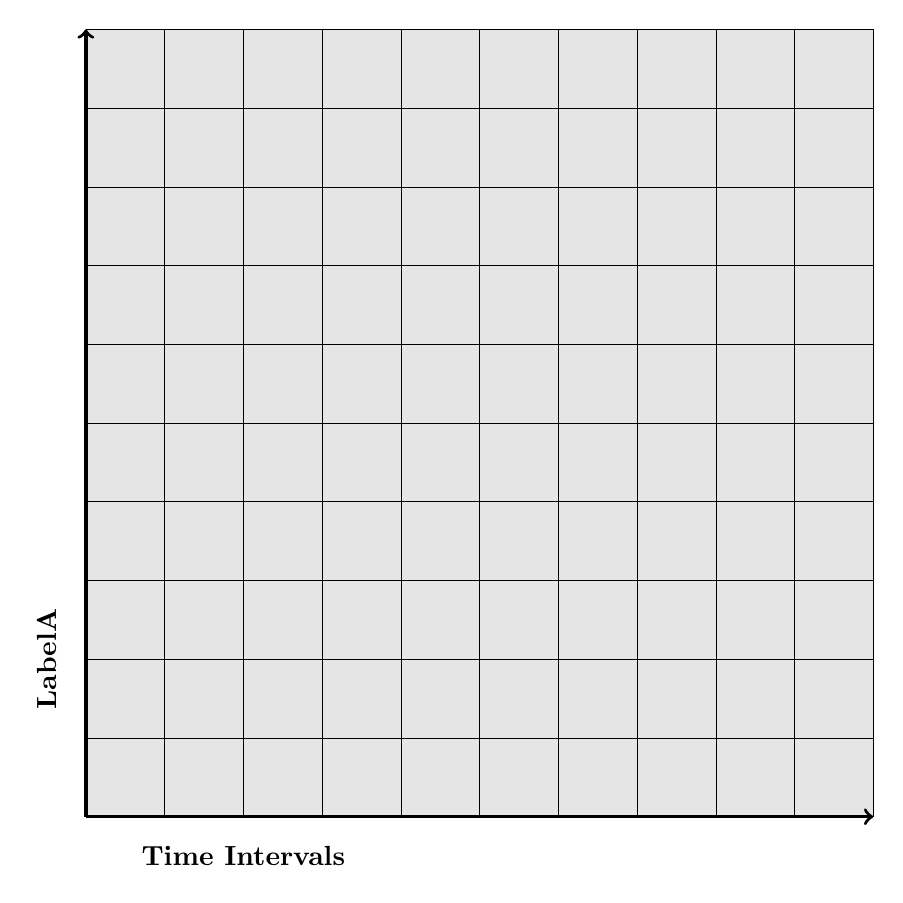
\begin{tikzpicture}
\fill [black!10!white] (0,0) rectangle (10,10);
\draw[step=1cm,black,very thin] (0,0) grid (10,10);
\draw[very thick,->] (0,0) -- (0,10);
\draw[very thick,->] (0,0) -- (10,0);
\draw (-0.5, 2) node[rotate=90] {\bf LabelA};
\draw (2, -0.5) node {\bf Time Intervals};
\end{tikzpicture}

A Time Series DB is an $N$ dimensional matrix.

Each time interval adds an $(N-1)$ dimensional slice to the matrix.  In this
    example each time interval adds 10 values.  In 3 dimensions, 100.  In 4,
    1,000 values are added.

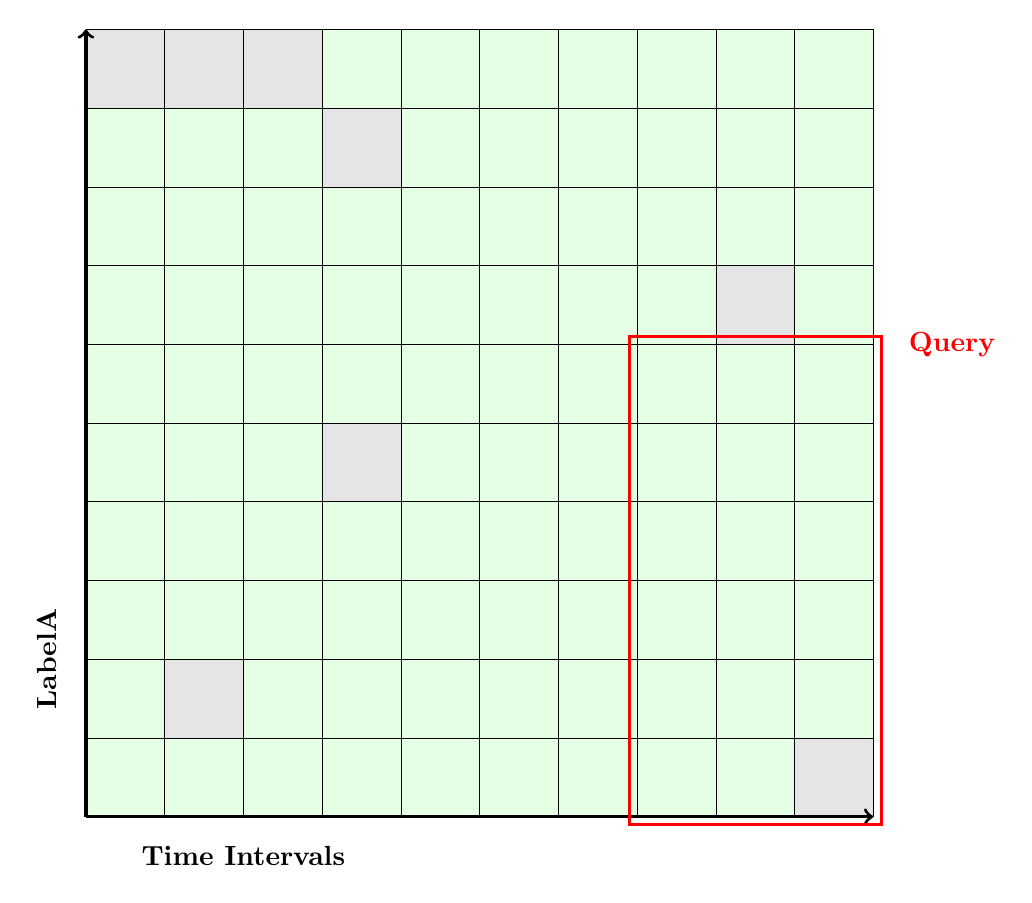
\begin{tikzpicture}
\fill [green!10!white] (0,0) rectangle (10,10);
\fill [black!10!white] (0,9) rectangle (3,10);
\fill [black!10!white] (1,1) rectangle (2,2);
\fill [black!10!white] (3,4) rectangle (4,5);
\fill [black!10!white] (3,8) rectangle (4,9);
\fill [black!10!white] (8,6) rectangle (9,7);
\fill [black!10!white] (9,0) rectangle (10,1);
\draw[step=1cm,black,very thin] (0,0) grid (10,10);
\draw[very thick,->] (0,0) -- (0,10);
\draw[very thick,->] (0,0) -- (10,0);
\draw (-0.5, 2) node[rotate=90] {\bf LabelA};
\draw (2, -0.5) node {\bf Time Intervals};

\draw[red, very thick] (6.9, -0.1) rectangle (10.1, 6.1);
\draw [red] (11, 6) node {\bf Query};
\end{tikzpicture}

Time Series DBs efficiently return a sub matrix in response to a query.  In the optimal case
the matrix is highly populated and queries are small and efficient.  This example query returns
17 values in a 3x8 sub matrix.

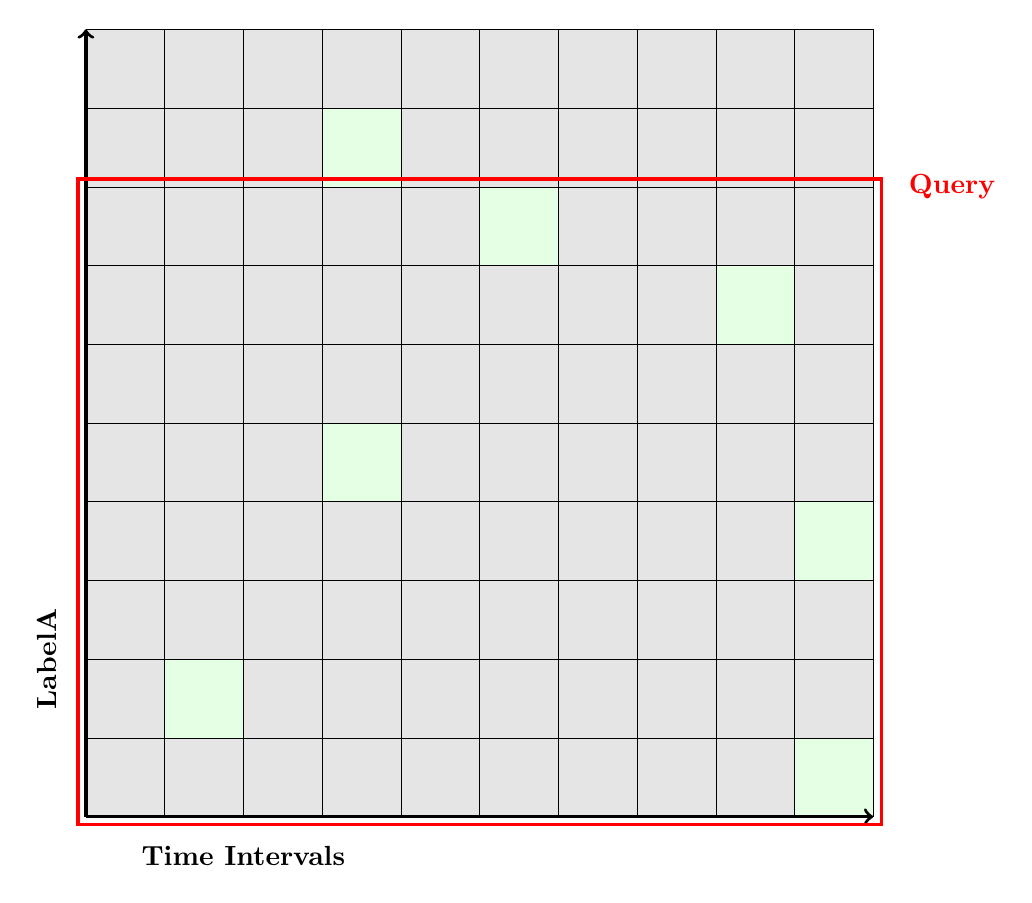
\begin{tikzpicture}
\fill [black!10!white] (0,0) rectangle (10,10);
\fill [green!10!white] (1,1) rectangle (2,2);
\fill [green!10!white] (3,4) rectangle (4,5);
\fill [green!10!white] (3,8) rectangle (4,9);
\fill [green!10!white] (8,6) rectangle (9,7);
\fill [green!10!white] (9,0) rectangle (10,1);
\fill [green!10!white] (5,7) rectangle (6,8);
\fill [green!10!white] (9,3) rectangle (10,4);
\draw[step=1cm,black,very thin] (0,0) grid (10,10);
\draw[very thick,->] (0,0) -- (0,10);
\draw[very thick,->] (0,0) -- (10,0);
\draw (-0.5, 2) node[rotate=90] {\bf LabelA};
\draw (2, -0.5) node {\bf Time Intervals};

\draw[red, very thick] (-0.1, -0.1) rectangle (10.1, 8.1);
\draw [red] (11, 8) node {\bf Query};
\end{tikzpicture}

In mathematics \textit{Cardinality} refers to the size of the set or matrix.  In Time Series DB operations
high cardinality implies that the matrix size is so large that the population of data tends
to be very sparse.
In this example a larger query selects a 10x8 sub matrix but only finds 6 real values.  Yet, all 80 possible values must be processed to find a result!

\end{center}
\end{document}
